\documentclass{beamer}

\usetheme{simple}

\usepackage{caption}
\usepackage{xcolor}
\usepackage{fancyvrb}
\usepackage{ulem}
\usepackage{subcaption}
\usetikzlibrary{positioning,calc,automata}

\title{CSC363 Tutorial \#6}
\subtitle{NTMs. \tiny Guess the meaning of this acronym.}
\date{March 2, 2022}
\institute{}

\newcommand{\N}{{\mathbb N}}
\newcommand{\R}{{\mathbb R}}
\newcommand{\inner}[1]{\langle #1 \rangle}

\setwatermark{
\includegraphics[height=8cm]{img/chungus.png}}

\begin{document}

\maketitle

\begin{frame}{Learning objectives this tutorial}
\begin{itemize}
\item Learn the formal definition of a Nondeterministic Turing Machine.
\item Understand how Nondeterministic TMs accept and reject inputs, and why this gives NTMs an unfair advantage over vanilla TMs.
\item Understand how, in the end, both NTMs and TMs are equivalent in some ways, but different in other ways.
\end{itemize}
\end{frame}

\begin{frame}{Assignment tips}
\begin{itemize}
\item Come to office hours! We may be able to drop some hints there.
\item Read Cooper's book! Although everything you need is covered in the slides, the book goes through it more slowly.\footnote{Personally, when learning the course material, I found Cooper's book to be extremely helpful.} The book contains many more examples.
\begin{itemize}
    \item Specifically, chapter 7 will really help with the assignment.
\end{itemize}
If you do not have the book, please, \textit{do not} try to download this illegally, such as through pirating.
\begin{figure}[h]
    \centering
    
\includegraphics[width=4cm]{img/trollge.png}
\end{figure}
\end{itemize}
\end{frame}

\begin{frame}{(Deterministic) Turing Machines}
\textbf{Task:} Fill in $\ldots$. \\

\vspace{2mm}

A Turing Machine is a 7-tuple $(Q, \Sigma, \Gamma, \delta, q_0, q_{\text{accept}}, q_{\text{reject}})$ where:
\begin{itemize}
    \item $Q$ is $\ldots$
    \item $\Sigma$ is $\ldots$
    \item $\Gamma$ is $\ldots$
    \item $\delta: \ldots \to \ldots$ is the transition function.
    \item $q_0$ is $\ldots$
    \item $q_{\text{accept}}$ is $\ldots$
    \item $q_{\text{reject}}$ is $\ldots$
\end{itemize}
\end{frame}

\begin{frame}{(Deterministic) Turing Machines}

A Turing Machine is a 7-tuple $(Q, \Sigma, \Gamma, \delta, q_0, q_{\text{accept}}, q_{\text{reject}})$ where:
\begin{itemize}
    \item $Q$ is the set of states.
    \item $\Sigma$ is the \textit{input alphabet}.
    \item $\Gamma$ is the \textit{tape alphabet} (and satisfies $\Gamma \subseteq \Sigma$).
    \item $\delta: (Q \times \Gamma) \to (Q \times \Gamma \times \{L, R\})$ is the transition function.
    \item $q_0$ is the starting state.
    \item $q_{\text{accept}}$ is the accept state.
    \item $q_{\text{reject}}$ is the reject state.
\end{itemize}
\end{frame}

\begin{frame}{(Nondeterministic) Turing Machines}

A Nondeterministic Turing Machine is a 7-tuple $(Q, \Sigma, \Gamma, \delta, q_0, q_{\text{accept}}, q_{\text{reject}})$ where:
\begin{itemize}
    \item $Q$ is the set of states.
    \item $\Sigma$ is the \textit{input alphabet}.
    \item $\Gamma$ is the \textit{tape alphabet} (and satisfies $\Gamma \subseteq \Sigma$).
    \item $\delta \subseteq (Q \times \Gamma) \times (Q \times \Gamma \times \{L, R\})$ is the transition relation.
    \item $q_0$ is the starting state.
    \item $q_{\text{accept}}$ is the accept state.
    \item $q_{\text{reject}}$ is the reject state.
\end{itemize}

\textbf{Task:} What changed, compared to the original Turing Machine definition?
\pause

\textbf{Ans:} $\delta$ is no longer a transition \textit{function}! It is a transition \textit{relation}.\footnote{Recall that a \textit{relation} $R$ between $A$ and $B$ is a subset of $A \times B$. A \textit{function} from $A$ to $B$ is a relation between $A$ and $B$ where for each $a \in A$, there exists a unique $b \in B$ such that $(a, b)$ is in the relation.
}
\end{frame}

\begin{frame}{(Nondeterministic) Turing Machines}

The difference between a NTM and TM can be viewed as parallel to the difference between a DFA and NFA (from CSC236). In a NTM's transition table, we may have multiple different transitions for the same state and same character. 

\pause
\vspace{2mm}

A NTM $M$ \textbf{accepts} input $x$ when $M$ has \textit{some} execution path that ends in $q_{\text{accept}}$. Otherwise:
\begin{itemize}
    \item If all execution path ends in $q_{\text{reject}}$, $M$ \textbf{rejects} input $x$.
    \item Otherwise, it loops.
\end{itemize}

\pause

In some sense, think of NTMs like job applications. If you have one job offer, you're good! Otherwise :(

\end{frame}

\begin{frame}{(Nondeterministic) Turing Machines}
A NTM $M$ \textbf{accepts} input $x$ when $M$ has \textit{some} execution path that ends in $q_{\text{accept}}$. Otherwise:
\begin{itemize}
    \item If all execution path ends in $q_{\text{reject}}$, $M$ \textbf{rejects} input $x$.
    \item Otherwise, it loops.
\end{itemize}

In some sense, think of NTMs like job applications. If you have one job offer, you're good! Otherwise :(

\begin{figure}[h]
    \centering
    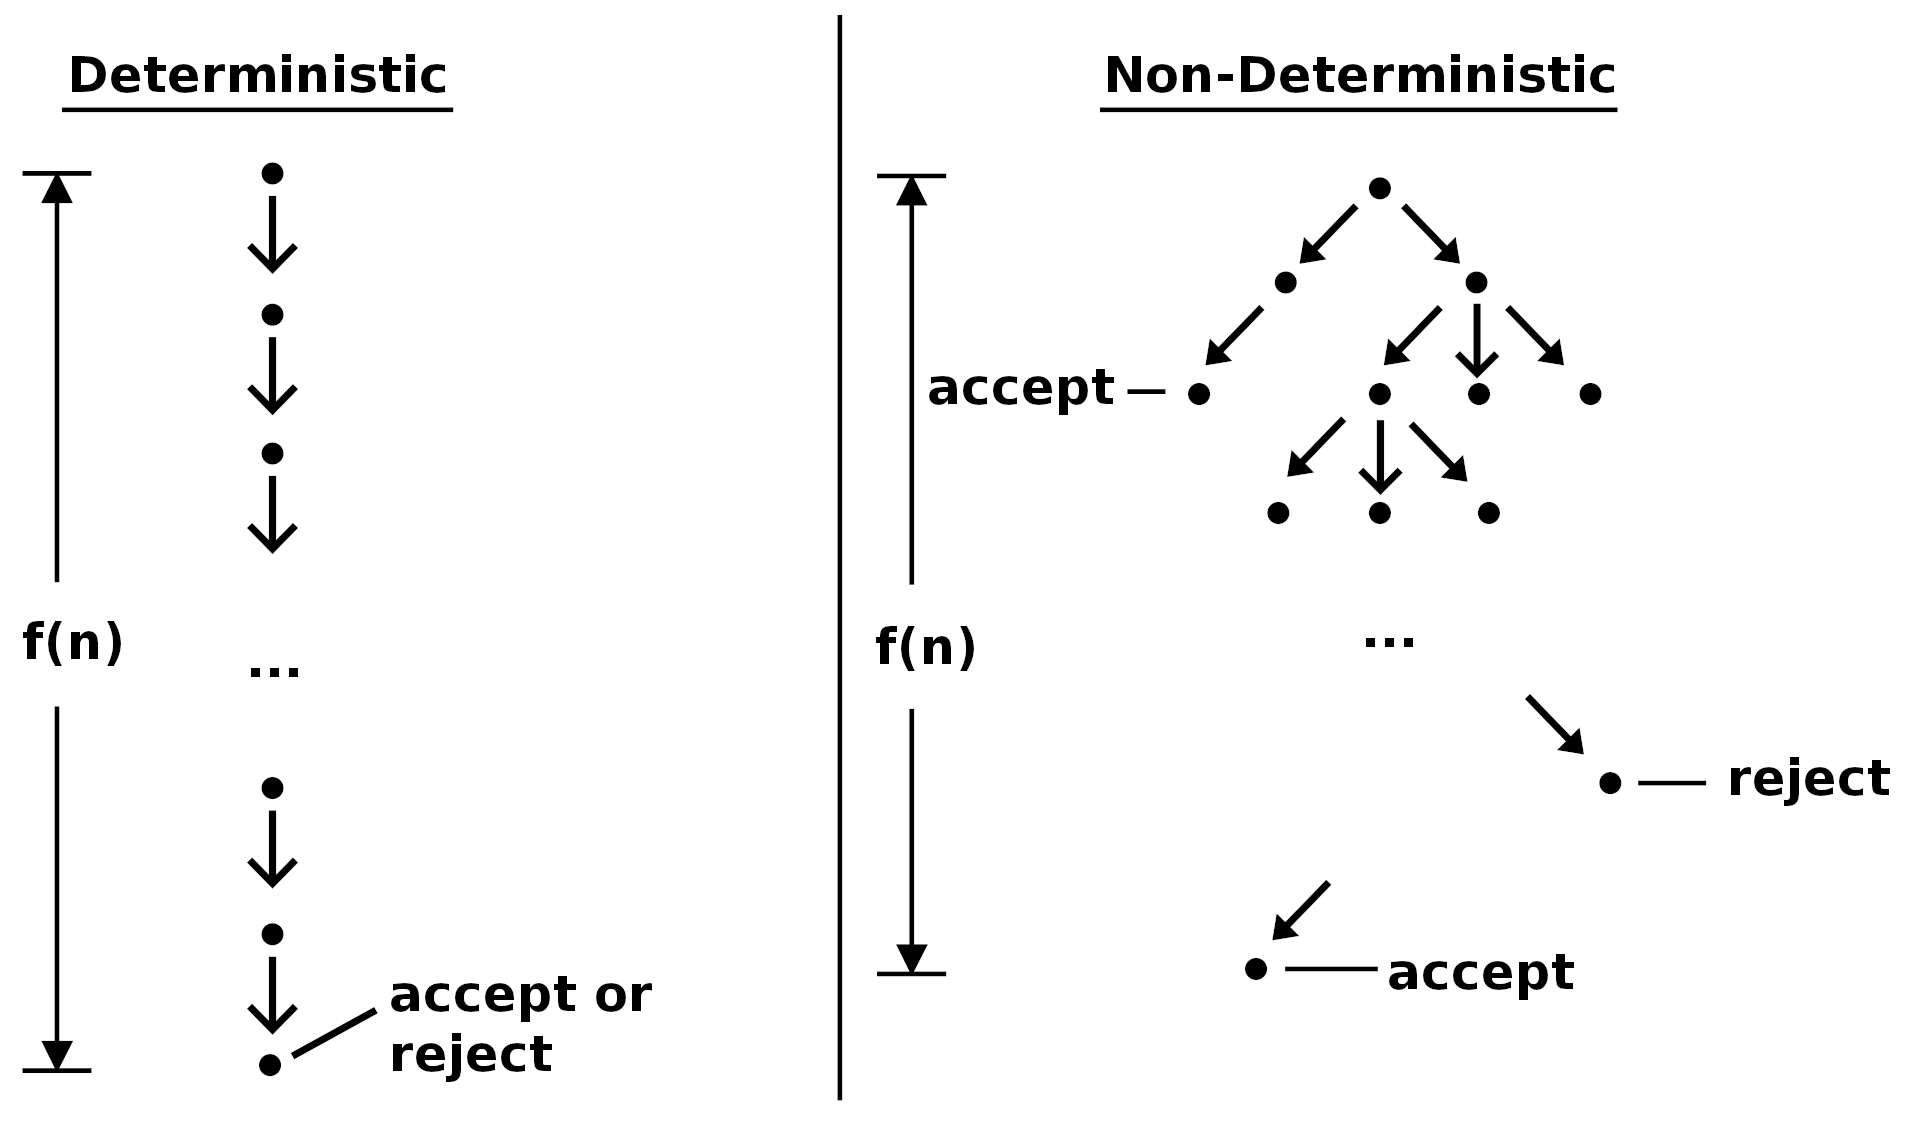
\includegraphics[height=4cm]{img/NTM.png}
\end{figure}
NTMs have multiple different ``execution paths''.
\end{frame}

\begin{frame}{Subset Sum}

\textbf{Task:} Let $S = \{5, 7, 11, 12, 14\}$. Can you find a subset $S' \subseteq S$ such that $S'$ sums to $24$? What about $27$?

\pause

\textbf{Ans:} There is a subset that sums to 24, namely $\{5, 7, 12\}$. There are no subsets that sum to $27$, on the other hand.

\vspace{2mm}

\pause

This is a specific case of the \textbf{subset sum problem}. Given a finite set of natural numbers $S$ and a \textit{target} $t \in \mathbb N$, can we find a $S' \subseteq S$ such that $S'$ sums to $t$?

\pause
\vspace{2mm}

\textbf{Task:} Write a function \texttt{subset\_sum(S, t)} that returns True iff $S$ has a subset that sums to $t$, using pseudocode.

\end{frame}

\begin{frame}[fragile]{Subset Sum}
\textbf{Task:} Write a function \texttt{subset\_sum(S, t)} that returns True iff $S$ has a subset that sums to $t$, using pseudocode.

\textbf{Ans:}
\begin{verbatim}
def subset_sum(S, t):
  for every subset S' of S:
    if S' sums to t:
      return True
  return False
\end{verbatim}

\textbf{Task:} What is the runtime of \texttt{subset\_sum(S, t)}, in terms of $|S|$ (the size of $S$)?
\pause \textbf{Ans:} It is $O(2^{|S|})$.

\begin{figure}[h]
    \centering
    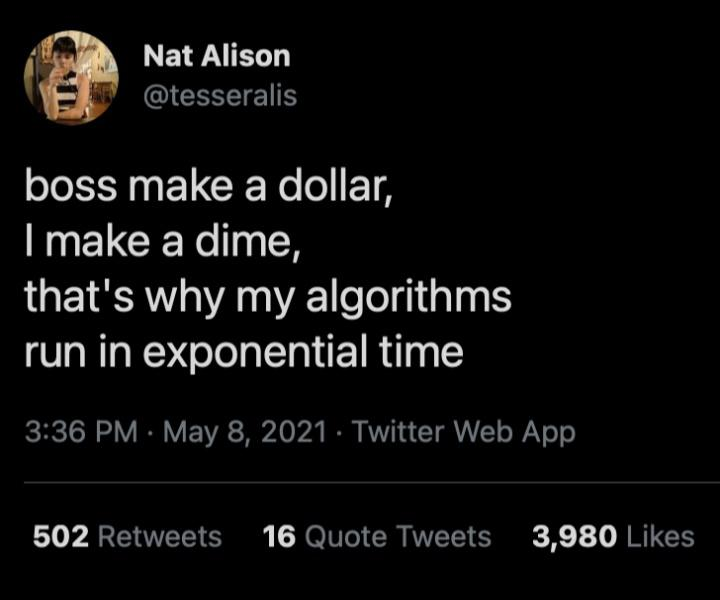
\includegraphics[height=3cm]{img/exp_time.jpg}
\end{figure}
\end{frame}

\begin{frame}{Subset Sum}
\textbf{Task:} Write a function \texttt{subset\_sum(S, t)} that returns True iff $S$ has a subset that sums to $t$, using pseudocode. Make sure to do it in polynomial time!

\textbf{Ans:}
\begin{figure}[h]
    \centering
    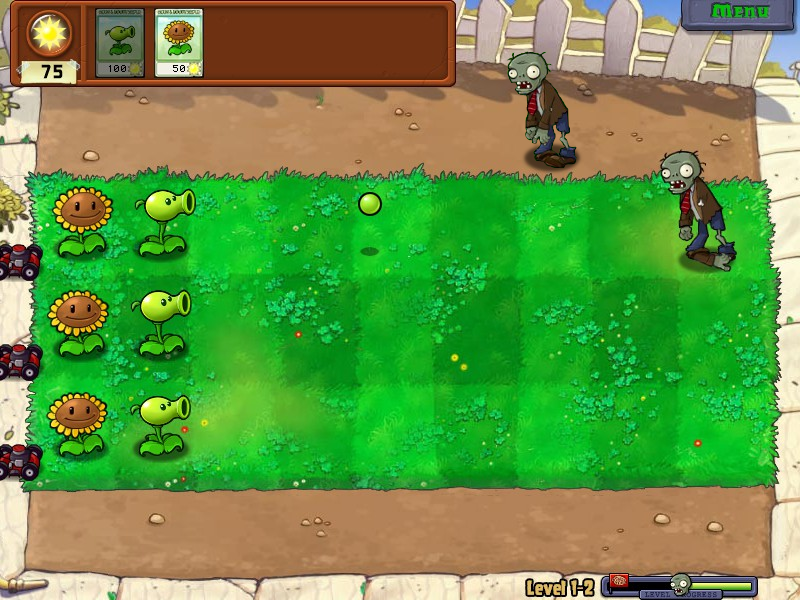
\includegraphics[height=6cm]{img/pvz.png}
    \caption*{(we don't know if it's possible or not)}
\end{figure}
\end{frame}

\begin{frame}[fragile]{Subset Sum}
Wait! What about the following code? Does this solve subset sum?

\begin{verbatim}
def subset_sum_2(S, t):
  choose a random subset S' of S
  if S' sums to t:
    return True
  return False
\end{verbatim}
\pause

Of course not! But \texttt{subset\_sum\_2} is not entirely useless. If we're lucky and \texttt{subset\_sum\_2} returns True, then indeed, there is a subset $S'$ that sums to $t$. If it returns False instead, we don't know anything...

\end{frame}

\begin{frame}[fragile]{Subset Sum}
This process of choosing a ``random'' $S'$ may be implemented in a NTM. The NTM will \textit{simultaneously choose all} particular subsets $S'$, and accept if and only if one execution path returns True.

\begin{verbatim}
def subset_sum_ntm(S, t):
  choose a particular subset S' of S
  if S' sums to t:
    return True
  return False
\end{verbatim}

And it runs in linear time (in terms of the maximum execution length)! Unfortunately we can't implement this in real life... :(

\begin{figure}[h]
    \centering
    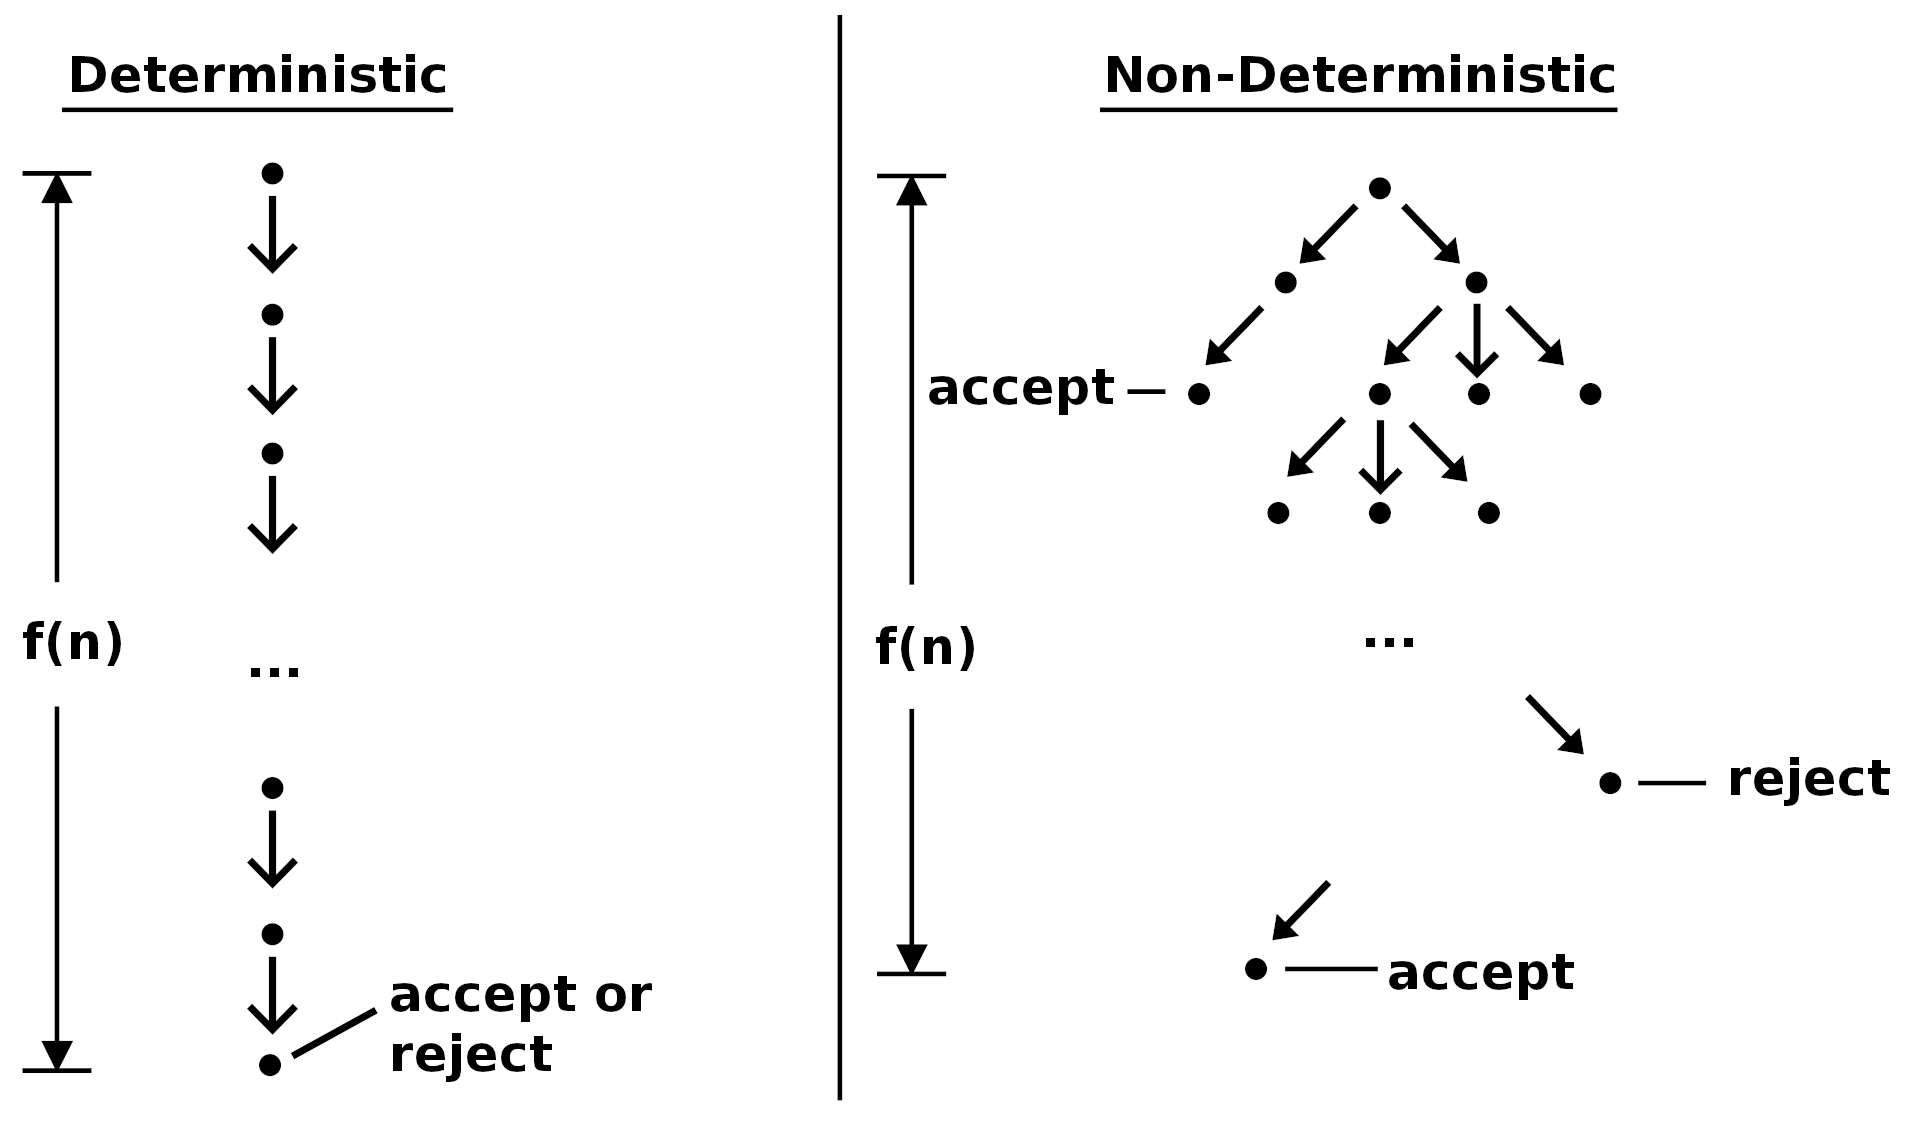
\includegraphics[height=2.5cm]{img/NTM.png}
    \caption*{$f(n)$ is the execution length.}
\end{figure}

\end{frame}

\begin{frame}[fragile]{Subset Sum}
\textbf{Conclusion}: The subset sum problem can be solved in linear time by a NTM. However, we don't know if we can solve the subset sum problem with a TM.\footnote{This amounts to solving the P = NP problem; we will explain how later in this course.} 

\pause

\textbf{Question:} Disregarding runtime, is there any problem that a NTM can solve, but a TM can't solve?

\pause

\textbf{Ans:} No! This is because we can simulate a NTM on a TM.

\begin{verbatim}
def simulate_NTM(ntm, input):
  while True:
    execute ntm(input) one step.
    if there are multiple possible transitions, 
    spawn a thread here to simulate each possible transition
\end{verbatim}

In the same way DFAs can recognize any languages that NFAs recognize, TMs can solve any problem that a NTM can solve (but the TM may be much slower).
\end{frame}



\end{document}